\documentclass[12pt]{article}
\usepackage{xdipp} % Replace 'mystyle' with the name of your .sty file

\begin{document}

% Your document content goes here

\titul
{Implementace evidence docházky pro elektronický docházkový systém Mendelovy univerzity v Brně}
{Andrey Chernenko}
{Ing. Oldřich Faldík, Ph.D.}
{Brno 2023}

\podekovani{
        Chtěl bych poděkovat svému vedoucímu Oldřichu Faldíkovi, 
    Ph.D., za jeho vedení a rady při vypracování této bakalářské práce. Jeho odborné 
    znalosti a rady byly pro mě velkou pomocí. Děkuji také rodině a 
    přátelům za jejich podporu během mého studia.
}


\prohlasenimuz
{Brno 21.9.2023}

\abstract{}{This bachelor thesis deals with the implementation of a reports component, 
    which is a part of attendance records in the Smart Mendelu environment. 
    The thesis also contains a general overview of the implementation of microservices 
    and examines the benefits and shortcomings of using a microservices architecture. 
    The solution was developed using the object-oriented programming language Java 
    and its Spring Boot framework, along with JavaScript and its Vue.js framework 
    to create a reactive user interface.
}
\abstrakt{}{Tato bakalářská práce se zabývá implementací komponenty sestavy, 
    která je součástí evidence docházky v prostředí Smart Mendelu. 
    Práce dále obsahuje obecný přehled problematiky implementace mikroslužeb 
    a zkoumá přínosy a nedostatky použití architektury mikroslužeb. 
    Řešení bylo vytvořeno s využitím objektově orientovaného programovacího jazyka Java 
    a jeho frameworku Spring Boot, spolu s JavaScriptem a jeho frameworkem Vue.js 
    pro vytvoření reaktivního uživatelského rozhraní.
}

\obsah
\cislovat{1}
\cislovat{2}


\kapitola{Úvod}
\sekce{Úvod do práce}
    Evidence docházky je důležitou součástí správy lidských zdrojů ve většině organizací různé
    velikostí. Elektronické docházkové systémy se staly běžnou cestou pro správu docházky,
    protože poskytují vysokou úroveň automatizace a přesnosti. Volba určitých nástrojů a
    architektur pro sestavení a zprovoznění aplikaci má své výhody a nevýhody. 
\sekce{Cíl práce}
    Cílem této práce je definovat problémy spojené s podstatou implementace evidence docházky a 
    vymezit funkční a nefunkční požadavky, které by tyto problémy pokryly. Během implementace 
    využit vyhod mikroservisní architektury na backendové straně a architektury jednostrankových 
    aplikací na frontendové straně. Budou představeny různé metody a technologie, které se používají 
    při vývoji informačních systémů.
\kapitola{Současný stav evidence docházky}
\sekce{Architektura}
Komponenta ED, která je využívána v současné době v produkčním prostředí, je postavena
na monolitické architektuře a napsána v skriptovacím jazyce PHP. Tento přístup zahrnuje:
\begin{itemize}
    \item Jednu základnu kódu
    \item Jednu databázi pro všechna data
    \item Jeden nebo několik serveru, na kterých běži instance aplikace
    \item Jeden bod vstupu pro všechny požadavky (index.php)
\end{itemize}

Výhody tohoto prístupu jsou v tom, že za prvé je jednoduchá a pochopitelná na
začátku vývoje. Za druhé je dobře škálovatelná v rámcí jednoho zařízení, protože základná
kódu se nachází na jednom místě. Ze stejného důvodu je snadno jí nasazovat, testovat a je
proto nákladově efektivní.
Evidence docházky není jedinou komponentou, která běží na serveru, spolu s ní
neoddělitelně běží i další částí aplikace. Během času kódová základna informačního systému
docházky se bude rozšiřovat, částí kódu se stanou na sobě více závislé. Kvůli tomu ladění a
oprava chyb, testování jednotlivých částí kódu, nasazení budou probíhat obtížněji, protože se
zvyšuje riziko poškodit program na jiném místě. Při škálování monolitického systému také
nastává problém protože pokud bude třeba oddělit a přenést na jiné zařízení určitou část
systému, to prakticky nebude uskutečnitelné.
\sekce{Návrh}
O vizualním designu aplikace. Body k zohlednění:
\begin{itemize}
    \item Jasnost a Srozumitelnost
    \item Přehlednost
    \item Responzivita
\end{itemize}
\sekce{Bezpečnost}
Body k zohlednění:
\begin{itemize}
    \item Zranitelnosti použitých knihoven
    \item Validace Vstupů
    \item Ochrana proti CSRF, XSS, SQL Injection
    \item Šifrování
\end{itemize}
\sekce{Výhody použití nových technologií}
    Podle nefunkčních požadavku popsaných v předchozí kapitole vyhovující
    architekturou na straně serveru bude architektura mikroslužeb. Podle Newmana (2015) mikroslužby jsou
    přístupem distribučních systémů které propagují použití dobře rozdělených služeb se
    samostatnými životními cykly, pro vzájemnou spolupraci. Mikroslužby mají několik výhod
    oproti monolitické architektuře, mezi nimi patří:
\sekce{Současné trendy vývoje webových aplikací}
    (ne)kratký přehled současných architektur a principů postavení aplikací
\begin{itemize}
    \item Škálovatelnost, díky které častí aplikaci se dá spustit nezávislé a na různých
    zařízeních.
    \item Odolnost: pokud z určitých důvodů komponenta přestane fungovat, ostatní
    komponenty zůstanou pokračovat v běhu.
    \item Znovupoužitelnost: v případě nadměrné zátěže na určitou komponentu lze tuto
    komponentu duplikovat a provést load balancing.
    \item Testování: jednotlivé mikroslužby je možné testovat nezávisle na ostatních.
    \item Jednoduchost vnímání a pochopení programu: v menší komponentě lze snadněji
    sledovat závislostí kódu.
\end{itemize}

\kapitola{Postup implementace}
\sekce{Backendová část}
Popís struktury Spring Boot aplikace: endpointy, napojení na databazi, použite nastroje/baličky
\sekce{Frontendová část}
Na začátku webové stránky představovaly sebou systémy, ve kterých na straně serveru probíhála uplná generace HTML stránek.
Server po obdržení požadavku se mohl dotazovat na externí API, ziskávat data z databaze a provádět interní zpracování těchto zkumulovaných dat. 
Následně shromažděná informace spolu s JavaScript funkcemi se dosazovala do výsledné HTML stránky a celá byla odesílana klientovi zpět. 
Jako každa metoda implementace webových stránek, tato metoda má svoje výhody, především z hlediska:
\begin{enumerate}
    \item procházení a indexování webu vyhledavači
    \item konzistenci a přístupnosti výsledné stránky bez ohledu na prezenci JavaScriptu u klienta. 
\end{enumerate}

\hspace{0.5cm} Jestli s benefitem číslo 1 ještě bychom mohli souhlasit, u druhého bodu už by se dalo tvrdit, že JavaScript je standardem každého prohližeče 
a s každým dnem do budoucna pravděpodobnost chyby v jeho jádru se snižuje. Výjimkou může být případ, kdy za účelem bezpečnosti spouštění JavaScriptu u klienta muže být omezeno nebo zcela zakázano, 
v takových případech posílaní potřebných funkcí ze serveru je jediná cesta ho použit. 
Je znam i další benefit tohoto přístupu, však také není tak jednoznačný -- rychlost renderování stránek. Postupem času webové stránky zvyšují svoji komplexitu,
jak z hlediska vypočtu potřebných dat, tak z hlediska visualního vzhledu. Vzhledem k tomu čas potřebný pro renderování neustalé roste, mezitím klientovi nic nezbývá 
než čekat na odpověď serveru.

\hspace{0.5cm} Skutečnost, že výpočetní zátěž je zcela ramenách serveru v případě populárních MVC frameworků je podle Mikovskeho a Powella je jedním z důvodů jejich pomalosti.
Alternativou tomuto tradičnímu přístupu je jednostránková aplikace (angl. Single Page Application, SPA). SPA je aplikace doručená do prohlížeče, která během používání znovu 
nenačítá stránku. Stejně jako všechny ostatní aplikace je určena k tomu, aby uživateli pomohla dokončit určitý úkol, například "napsat dokument" nebo "spravovat webový server". 
SPA si můžeme představit jako tlustého klienta, který se načítá z webového serveru.

\sekce{Framework Vue.js}
Vue.js je framework napsany v JavaScriptu a jeho hlavním použitím je implementace uživatelského rozhrání. 
Je postaven nad standartní programovací soupravou jazyků HTML, CSS a JavaScript. 
Model programování je záložen na komponentově-deklarativním přístupu. V nasledijicích obrazcích si ukážeme příklad, 
ve kterém rozhrání aplikace Sestavy se přepíná z české na anglickou lokalizaci: 
\begin{figure}[H]
    \centering
    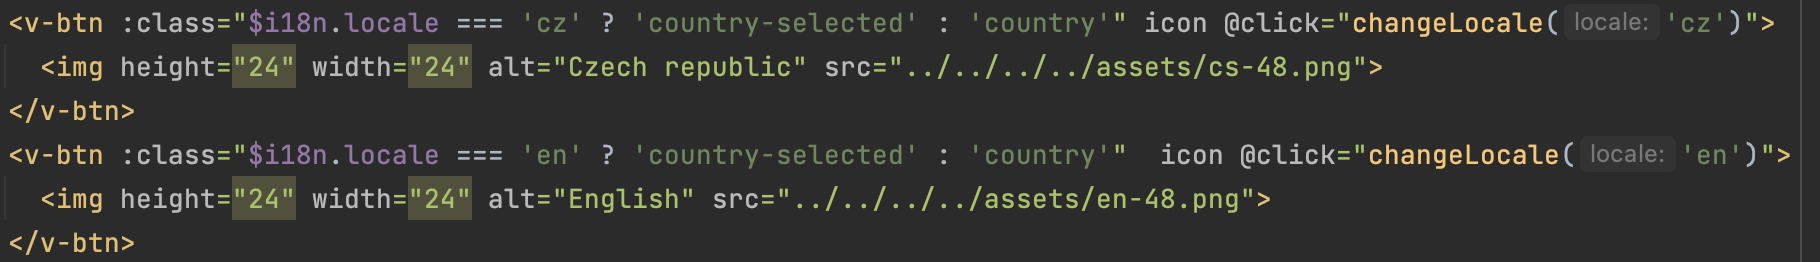
\includegraphics[width=0.8\textwidth]{images/_lokalizace.png}
    \caption{Zdrojové kod tlačitek lokalizace}
\end{figure}
\begin{figure}[H]
    \centering
    
\includegraphics[width=0.8\textwidth]{images/en_lokalizace.png}
    \caption{Výchozí nastavení lokalizace}
\end{figure}
\begin{figure}[H]
    \centering
    
\includegraphics[width=0.8\textwidth]{images/cz_lokalizace.png}
    \caption{Změna lokalizace na českou}
\end{figure}
Příklad výše ukazuje dvě klíčové vlastností tohoto přístupu:
\begin{itemize}
    \item Deklarativní vykreslování: Vue rozšiřuje standardní HTML o syntaxi šablon, která nám umožňuje deklarativně popsat výstup HTML na základě stavu JavaScriptu.
    \item Reaktivita: Vue automaticky sleduje změny stavu JavaScriptu a při změnách efektivně aktualizuje DOM.
\end{itemize}











Popís struktury Vue.js aplikace: implementace vizualních komponent
(tabulky, uživatelský panel), autentikace, použite nastroje/baličky.
\newline
\newline
Poznámky:
\begin{itemize}
    \item Konfigurace adapteru pro identity management nástroj Keycloak, vlastní plugin Auth pro Vue
    \item Cross-site request forgery https://security.stackexchange.com/questions/20187/oauth2-cross-site-request-forgery-and-state-parameter
    \item Balik vue-router pro routing v SPA aplikacích, princip routování u spa aplikací
    \item State management plugin Vuex pro framework Vue

\end{itemize}

\end{document}
